% Copyright (C) 2019 Cui Jialiang ( SESS, PKU ). All rights reserved.

\chapter{基于Tensorflow的像素级视频目标跟踪实验}
为了验证本研究提出的方法的可行性和价值,我们设计了一个实验。后文中该实验将被称为本实验。本实验基本实现了本研究提出的方法,并得到了一定的结果和结论.
\par
本章接下来的部分将介绍本实验的设计思路,硬件环境和数据等实验条件,实验代码的实现和实验结果的评估方法。

\section{实验总体设计思路}
类似于大多数算法研究,本研究以计算机软件的形式实现了本研究提出的算法,并选择数据进行了实验.

\section{实验软硬件环境}
\subsection{软件环境}
本实验的软件部分主要在Tensorflow\supercite{abadi2016tensorflow}框架下实现。
\par
Tensorflow是最初由谷歌公司开发的一套现以开源的机器学习框架,可以为算法研究者提供屏蔽操作系统与硬件,资源分配,梯度计算等功能,让研究者能将更多的注意力集中在算法过程中.对于本研究,Tensorflow主要贡献了CNN,RNN单元的结构定义,损失函数定义,正向反向传播与梯度更新等功能.

\subsection{硬件环境}
\par
需要说明的是本研究提出的算法可以部署在普通计算机上,也有希望部署在更快速,更低成本的FPGA等嵌入式平台上.本实验为了容易进行,目前只在PC(个人计算机)上进行.
\par
本实验所有的运算操作是在一台配置有英伟达GTX1070图形处理器,英特尔i7中央处理器,24GB内存的笔记本电脑上进行的。
\par
本实验深度学习计算部分使用了GPU加速,直接依赖Tensorflow的GPU选项进行。本研究曾尝试过只用CPU进行计算,也能得到一定结果。
\par
如果有更好的硬件条件(更多、更好的图形处理器,更大的内存,更多核心的CPU),本实验有希望会得到更精细的结果。

\section{实验数据}
本实验使用VOT2016数据集\supercite{Vojir-TR-2017-01}实现,相似的数据集还有VOT2017等。
\par
\begin{figure}[htbp!]
    \centering
    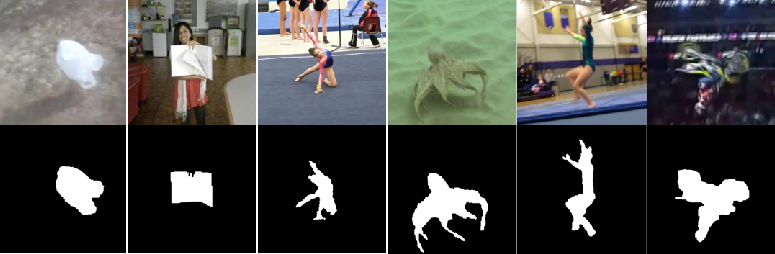
\includegraphics[width = 1.\textwidth]{chap/img/vot_2016_pixel.png}
    \caption{VOT2016像素级标记}\label{fig:vot_2016_pixel}
\end{figure}
\par
如图\ref{fig:vot_2016_pixel}所示,该数据集通过人工标记,提供了十分优秀的像素级的目标跟踪数据。该数据集有几百个序列,共有几万张图片。
\par
本实验的训练集和测试集均来源于该数据集,使用时将所有数据随机切分为训练集和测试集。


\section{实验程序的编写}
事实上,虽然借助于Tensorflow实现了许多计算功能,但本研究依然经历了许多代码开发工作,包括且不限于神经网络结构定义,训练数据处理等.
\par
本实验现先定义了CRNN的结构,即输入一个时间序列的序列图像,经过CRNN卷机循环网络得到另一个结果时间序列.在本实验的程序中,该结构可以选择使用LSTM或普通RNN单元.
\par
在加密-解码结构中,本实验定义了一个通用的层级结构,可以重复使用多次.如重复3次即是3层加密-解码结构.

\section{实验结果的评估方式}
由于像素级的视频目标跟踪算法缺乏评估体系,

\subsection{分类问题评估:精确度与准确度}
\subsection{分类问题评估:AUC}